\documentclass{article}
\usepackage[utf8]{inputenc}
\usepackage{multicol}
\usepackage{amsmath}
\usepackage{float}
\usepackage{epsfig,graphicx}
\usepackage{xcolor,import}
\usepackage{subcaption}
\usepackage[font=small,labelfont=bf]{caption}
\usepackage{siunitx}
\usepackage[german]{babel}
\usepackage{textcomp}
\usepackage{mathtools}

\begin{document}


\thispagestyle{empty}
			\begin{center}
			\Large{Fakultät für Physik}\\
			\end{center}
\begin{verbatim}


\end{verbatim}
							%Eintrag des Wintersemesters
			\begin{center}
			\textbf{\LARGE SOMMERSEMESTER 2015}
			\end{center}
\begin{verbatim}


\end{verbatim}
			\begin{center}
			\textbf{\LARGE{Physikalisches Praktikum II}}
			\end{center}
\begin{verbatim}




\end{verbatim}

			\begin{center}
			\textbf{\LARGE{PROTOKOLL}}
			\end{center}
			
\begin{verbatim}





\end{verbatim}

			\begin{flushleft}
			\textbf{\Large{Experiment (Nr. 6, Strahlung)}}\\
							%Experiment Nr. und Titel statt den Punkten eintragen
			\LARGE{}	
			\end{flushleft}

\begin{verbatim}

\end{verbatim}	
							%Eintragen des Abgabedatums, oder des Erstelldatums des Protokolls
			\begin{flushleft}
			\textbf{\Large{Datum:}} \Large{}
			\end{flushleft}
			
\begin{verbatim}
\end{verbatim}
							%Namen der Protokollschreiber
		\begin{flushleft}
			\textbf{\Large{Bachleitner Veronika, Grafendorfer Erik}} 
			\end{flushleft}

\begin{verbatim}


\end{verbatim}
							%Kurstag und Gruppennummer, zb. Fr/5
			\begin{flushleft}
			\textbf{\Large{Kurstag/Gruppe:}} \Large{FR/1}
			\end{flushleft}

\begin{verbatim}

\end{verbatim}
							%Name des Betreuers, das Praktikum betreute.
			\begin{flushleft}
			\LARGE{\textbf{Betreuer:\Large{ }}}		
			\end{flushleft}
\newpage
			
\section{Aufgabenstellung}
%Im ersten Experiment bestimmen wir das Planck'sche Wirkungsquantum.
\section{Theorie}
\subsection{Planck'sches Wirkungsquantum}
Beim Fotoeffekt werden elektrisch geladene Teilchen aus Materie angeregt (in einen höheren Energiezustand gebracht) oder freigesetzt, wenn sie von elektromagnetischen Wellen bestrahlt wird.\\
Bei der Anregung spricht man vom \textit{Inneren Fotoeffekt}, bei Freisetzung von Elektronen vom \textit{Äußeren Fotoeffekt}. Letzteres kommt bei Metallen vor, bei denen man die Leitungselektronen als frei in einem Potentialtopf beweglich beschreiben kann. Werden sie mit Energie größer gleich der notwendigen Austrittsarbeit angeregt, können die Elektronen sich aus dem Metall lösen.\\
\\
Einstein-Formel:
$$h\cdot\nu=A+E_{kin}=A+\frac{mv^2}{2}=A+eU_0$$


\subsection{Wärmestrahlung}
Das Planck'sche Strahlungsgesetz ist wie folgt gegeben:
\begin{equation}
L(\lambda,T)d\lambda = \frac{2hc^2}{\lambda^5} \cdot \frac{1}{\exp\left(\frac{hc}{\lambda kT}\right) -1} d\lambda
\label{strahlungsgesetz}
\end{equation}
wo $L(\lambda,T)d\lambda$ die gerichtete spektrale Strahldichte, abhängig von Wellenlänge und Temperatur. $L$ hat die Einheit $\frac{W}{m^2}\frac{sr}{nm}$.\\
\\

$$\frac{P_1}{P_2} = \frac{T_1^4}{T_2^4}$$
wo $P_i$ die zugeführte elektrische Leistung und $T_i$ die Temperatur.
$$\ln \frac{I_1}{I_2} = \frac{1}{T_1} \left(\sqrt[4]{\frac{P_1}{P_2}}-1\right) \cdot \frac{ch}{k\lambda}$$
wo $I_i$ die Lichtstärke
$$\frac{I_1}{I_2} = \frac{r_2^2}{r_1^2}$$
wo $I_i$ die Lichtstärken und $r_i$ die Abstände von der Lichtquelle.


\section{Aufbau}
\subsection{Planck'sches Wirkungsquantum}
Wir verwenden eine Quecksilberdampflampe, eine Fotozelle in einem geerdeten Metallzylinder (Fotokathode und Anodenring) und ein Pikoamperemeter zur Detektion des Fotostroms.

\subsection{Wärmestrahlung}
Für den Versuch verwenden wir eine Glühlampe, einen Interferenzfilter (um monochromatisches Licht zu erzeugen, $\lambda=560\si{nm}$ und eine Fotozelle. Außerdem einen Strom-Spannungswandler, um den in der Fotozelle erzeugten Strom messen zu können.

\section{Durchführung}
\subsection{Planck'sches Wirkungsquantum}
\subsection{Wärmestrahlung}


\section{Ergebnisse}
\subsection{Planck'sches Wirkungsquantum}
%Messen Sie den Fotostrom I als Funktion der Gegenspannung U im Bereich von 0-2V für fünf verschiedene Frequenzen und stellen Sie I gegen U in einem Diagramm graphisch dar.
%Führen Sie die Messung mit jedem der beiliegenden fünf dielektrischen Interferenzfilter durch. 
%Tragen Sie $\sqrt{I-I_0}$ gegen $U$ auf und extrapolieren Sie eine Gerade zum Schnittpunkt mit der U-Achse. Lesen Sie die damit eindeutig definierte Gegenspannung $U_0$ ab.

\begin{table}[H]
\begin{center}
\begin{tabular}{|c||c|c|}
\hline
$\nu$ ($10^{14}$Hz) & $U$ & $I$\\
\hline
$5.187$ &  &\\
 & &\\
$5.521$ & &\\
 & &\\
$6.908$ & &\\
 & &\\
$7.366$ & &\\
 & &\\
$8.213$ & &\\
 & &\\
\hline
\end{tabular}
\caption{Fotostrom $I$ und Gegenspannung $U$ bei 5 verschiedenen Frequenzen $\nu$.}
\end{center}
\end{table}

Gerade für $\nu=5.187$\\
$Ax+B=(-2.1 \pm 0.1)x+(0.57 \pm 0.01)$\\
%R^2=0.989
$x=0.27 \pm 0.05$\\ %0.05
$Ax+B=(-2.2 \pm 0.1)x+(0.58 \pm 0.01)$\\
%R^2=0.992
$x=0.26 \pm 0.05$\\
(mit einem Fit-Punkt weniger)\\
\\
Gerade für $\nu=5.521$\\
$(-7.0 \pm 0.2)x + (1.94 \pm 0.02)$\\
$x=0.28 \pm 0.03$\\ %Gauß: $\pm 0.03037$
%R^2=0.995
$(-7.2 \pm 0.2)x + (1.95 \pm 0.02)$\\
$x=0.27 \pm 0.03$\\ %Gauß: $\pm 0.0296$
%R^2=0.996
\\
Gerade für $\nu=6.908$\\
$(-8.39 \pm 0.01)x + (4.5637 \pm 0.0008)$\\
$x=0.5439 \pm 0.001$\\
%R^2=0.997
$(-8.62 \pm 0.01)x + (4.5874 \pm 0.0008)$\\
$x=0.532181 \pm 0.001$\\
%R^2=0.999

Gerade für $\nu=7.366$\\
$(-5.94 \pm 0.01)x + (3.50866 \pm 0.0006)$\\
$x=0.59068 \pm 0.0017$
%R^2=0.996
$(-6.11 \pm 0.01)x + (3.525857 \pm 0.0007)$\\
$x=0.577063 \pm 0.0016$
%R^2=0.997

Gerade für $\nu=8.213$\\
$(-13.17 \pm 0.01)x + (10.301904 \pm 0.0007)$
$x=$
%R^2=0.996
$(-13.76 \pm 0.01)x + (10.38 \pm 0.001)$
$x=$
%R^2=0.998

%Bestimmen Sie zu jeder Frequenz (Wellenlänge) die Gegenspannung $U_0$, bei der die schnellsten Elektronen den Anodenring gerade nicht mehr erreichen.
%Stellen Sie in einem Diagramm die Gegenspannung $U_0$ gegen die Frequenz $\nu$ dar. Führen Sie ein lineare Regression durch und bestimmen Sie die Austrittsarbeit $A$ und das Planck'sche Wirkungsquantum $h$. Entnehmen Sie aus dem Diagramm bei $U_0=0$ die untere Grenzfrequenz $\nu_g$.


\begin{table}[H]
\begin{center}
\begin{tabular}{|c|c|}
\hline
$\nu$ & $U_0$\\
\hline

\hline
\end{tabular}
\caption{}
\end{center}
\end{table}

%Stellen Sie entsprechend der Einsteingleichung die Spannung $U_0$ als Funktion der Frequenz $\nu$ graphisch dar und bestimmen Sie das Planck'sche Wirkungsquantum $h$, die Austrittsarbeit $A$ der Fotokathode und die untere Grenzfrequenz $\nu_g$.

Einstein-Formel:
$$h\cdot\nu=A+E_{kin}=A+eU_0$$
Da wir $e$ und $\nu$ kennen und $U_0$ messen können wir mit dieser Formel auf das Planck'sche Wirkungsquantum $h$ und die Austrittsarbeit $A$ schließen.\\
\\
Die Elementarladung $e=1.602177 \cdot 10^{-19}C$, die Lichtgeschwindigkeit $c=2.99792 \cdot 10^8 m/s$, die Masse des Elektrons $m=9.10939 \cdot 10^{-31}kg$, die Boltzmannkonstante $k=1.38066 \cdot 10^{-23}J/K$.

\begin{figure}
\centering
\begin{subfigure}{0.45\textwidth}
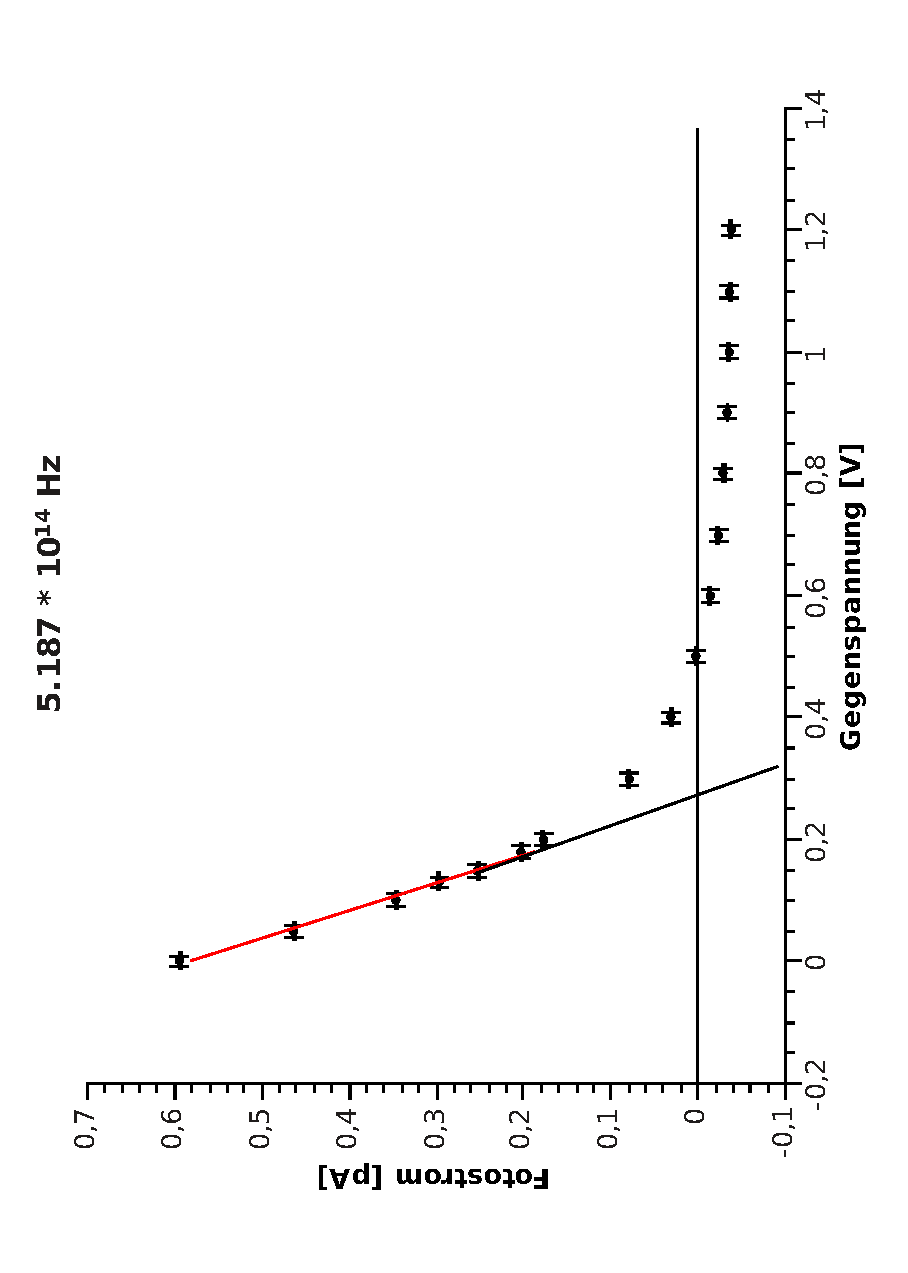
\includegraphics[width=\textwidth, angle=-90]{5187.eps}
\end{subfigure}
\hfill	
\begin{subfigure}{0.45\textwidth}
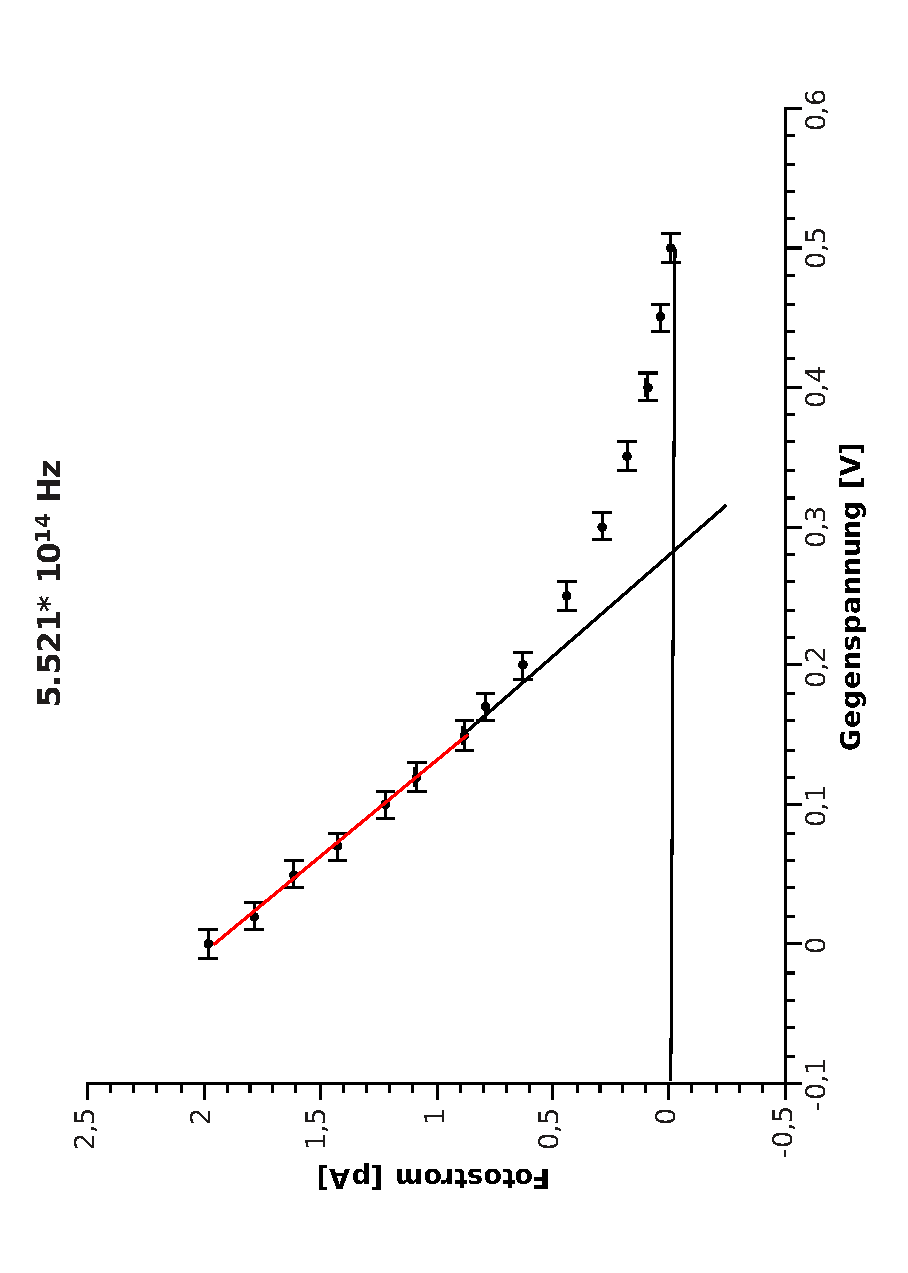
\includegraphics[width=\textwidth, angle=-90]{5521.eps}
\end{subfigure}
\begin{subfigure}{0.45\textwidth}
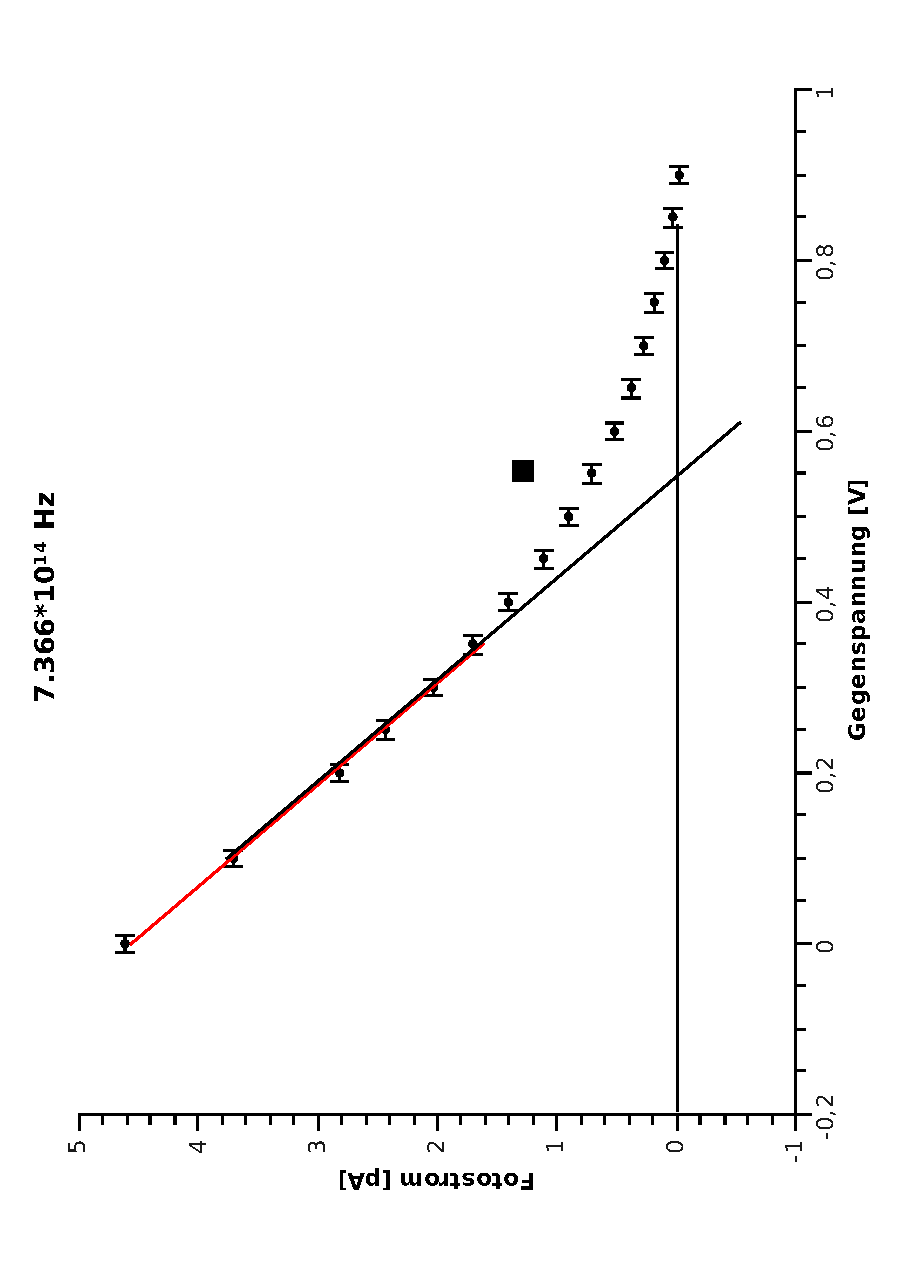
\includegraphics[width=\textwidth, angle=-90]{7366.eps}
\end{subfigure}
\hfill	
\begin{subfigure}{0.45\textwidth}
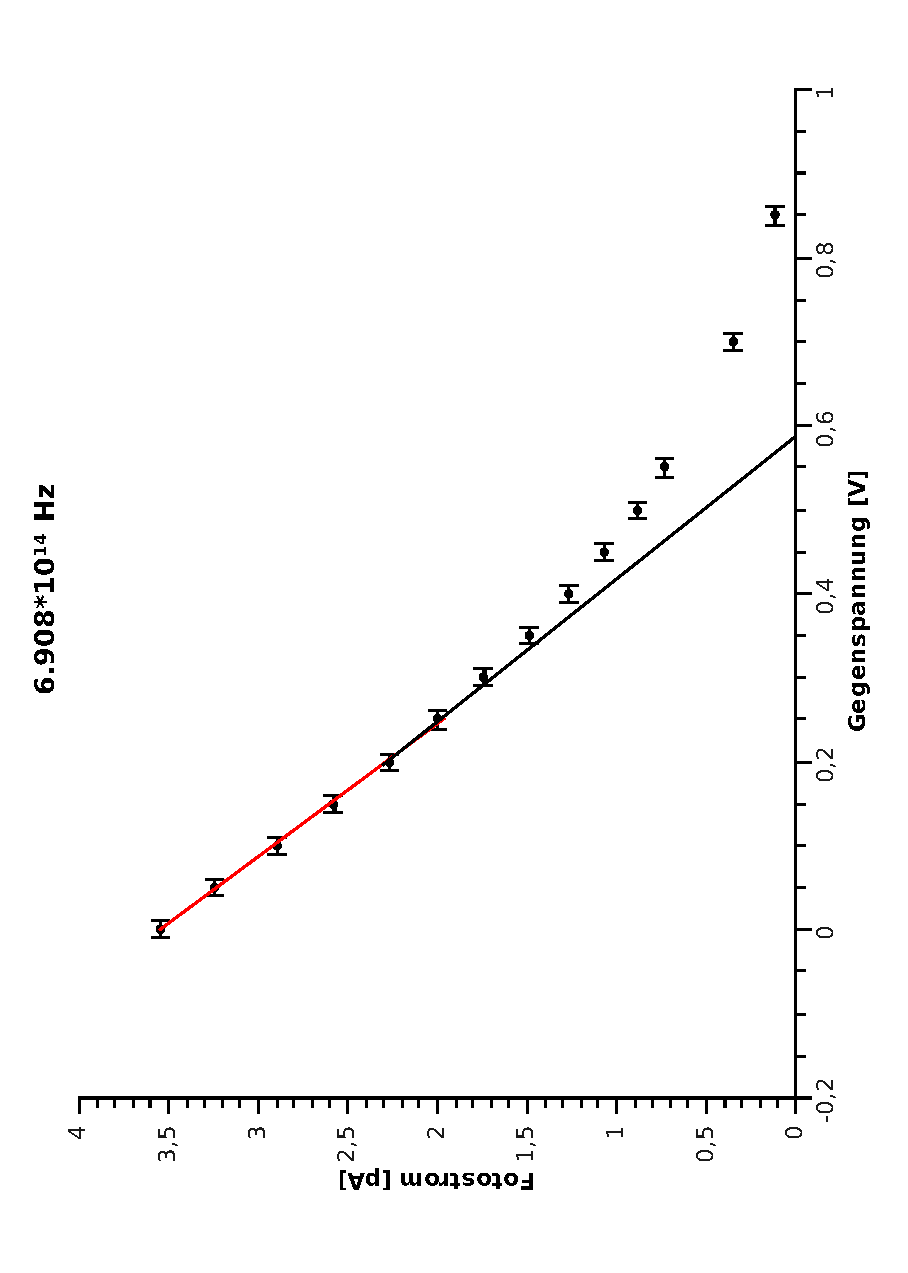
\includegraphics[width=\textwidth, angle=-90]{6908.eps}
\end{subfigure}
\begin{subfigure}{0.45\textwidth}
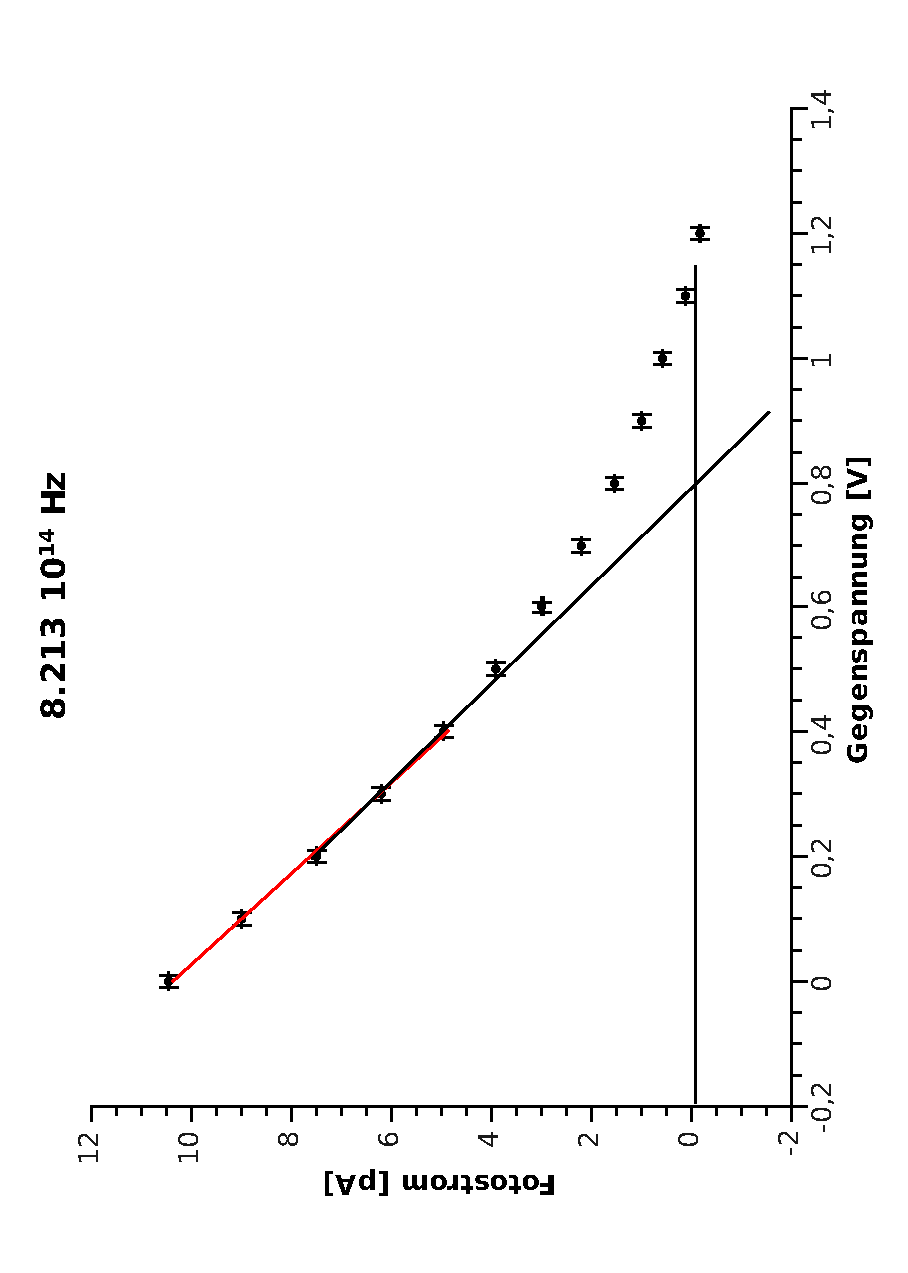
\includegraphics[width=\textwidth, angle=-90]{8213.eps}
\end{subfigure}
\end{figure}

\subsection{Wärmestrahlung}
%Tragen Sie in einem Diagramm die der Beleuchtungsstärke proprotionale Spannung in mV gegen $\frac{1}{r^2}$ für zwei Betriebsbedingungen (vom Betreuer erfragen) der Glühlampe auf. 14

%Abstand Ablesemarke - strahlende Fläche: $38\pm 1 \si{mm}$\\
%Abstand Ablesemarke - Fotozelle: $17.5 \pm 0.5 \si{mm}$\\
%Der Abstand r soll den Wert 50cm nicht unterschreiten.\\
Glühlampe steht anfangs auf 2cm.
Modus A: $I=(3.82 \pm 0.01)A$, $U=(3.65 \pm 0.01)V$\\
Modus C: $I=(4.81 \pm 0.01)A$, $U=(5.63 \pm 0.01)V$\\
\begin{table}[H]
\begin{center}
\begin{tabular}{|c|c|c|}
\hline
$r$ (cm) & $U_A$ (mV $\pm$ 1mV) & $U_C$ (mV $\pm$ 1mV)\\
97 & 49 & 259 \\
92 & 54 & 289 \\
87 & 59 & 321 \\
82 & 65 & 360 \\
77 & 75 & 410 \\
72 & 86 & 473 \\
67 & 100 & 553 \\
62 & 118 & 657 \\
57 & 142 & 793 \\
52 & 167 & 982 \\
\hline
\hline
\end{tabular}
\caption{Spannung an der Fotozelle und Abstände $r$ von der Glühlampe für zwei verschiedene Bestriebsbedingungen.}
\end{center}
\end{table}

%Bestimmen Sie die jeweils zugehörigen elektrischen Leistungen $P_1$ und $P_2$.

%Berechnen Sie für beide Betriebsbedingungen die Strahlungstemperaturen der Glühlampe. 12 und 13

$$\frac{P_1}{P_2} = \frac{T_1^4}{T_2^4}$$
$$\ln \frac{I_1}{I_2} = \frac{1}{T_1} \left(\sqrt[4]{\frac{P_1}{P_2}}-1\right) \cdot \frac{ch}{k\lambda}$$
$$\frac{I_1}{I_2} = \frac{r_2^2}{r_1^2}$$

\section{Diskussion}
\subsection{Planck'sches Wirkungsquantum}
Es fällt auf dass der Fotostrom mit der Frequenz des einfallenden Lichts steigt.
\subsection{Wärmestrahlung}
																								
\end{document}
